% FILE: main.tex  Version 2.1
% AUTHOR:
% Universit�t Duisburg-Essen, Standort Duisburg
% AG Prof. Dr. G�nter T�rner
% Verena Gondek, Andy Braune, Henning Kerstan
% Fachbereich Mathematik
% Lotharstr. 65., 47057 Duisburg
% entstanden im Rahmen des DFG-Projektes DissOnlineTutor
% in Zusammenarbeit mit der
% Humboldt-Universitaet zu Berlin
% AG Elektronisches Publizieren
% Joanna Rycko
% und der
% DNB - Deutsche Nationalbibliothek

\chapter{Discourse-Aware Sentiment Analysis}

Albeit coarse-grained seniment methods do a fairly good job at
classifying the overall polarity of a message, and DL-based approaches
also try their best to incorporate the compositional principle into
that prediction, a crucial limitation of all these systems is that
they overlook the structural nature of their input by either
considering it as a single whole (for example, of-features approaches)
or analyzing it as a monotone sequence of equally important elements
(for instance, recurrent neural methods).  Unfortunately, both of
these solutions completely ignore the hierarchical nature of language
\cite{Saussure:90,Hjelmslev:70}, in which morphemes are put together
to form words, words are united together into sentences, and multiple
sentences constitute a discourse.  Moreover, apart from this inherent
linguistic hierarchy, even units of the same language level might play
different roles and be of different importance while joined
syntagmatically: \eg{} in words, the root morpheme typically has more
lexical meaning than the affixes; in sentences, the syntactic head
grammatically dominates all its dependents.  The same kind of
structure can also be obsered in discourse, where one of the sentences
might express the gist of the whole text, but its meaning can still be
changed or reversed by other clauses.

Exactly the lack of the discourse information was the main reason for
the misclassifications of the systems of \citet{Severyn:15},
\citet{Baziotis:17}, and our own LBA method shown in Examples
\ref{snt:cgsa:exmp:severyn-error}, \ref{snt:cgsa:exmp:baziotis-error},
and \ref{snt:cgsa:exmp:lba-error} of the previous chapter.  Since none
of these approaches explicitly took the discourse structure into
account (in the best case, the inference simply proceeded from the
level of words directly to the level of message), we decided to check
whether making the last of these solutions (the LBA classifier) aware
of the discourse phenomena would improve its results.  However, before
we begin with our experiments, we should first give a short
introduction to the most popular approaches to discourse analysis in
the literature and justify our choice of one of them.  Afterwards, in
Section~\ref{sec:dasa:data}, we will describe the way of adding
discourse information to the existing PotTS and SB10k data.  Then, in
Section~\ref{sec:dasa:data}, we present a concise survey of the
existing discourse-aware sentiment analysis methods and evaluate their
results on the two aforementioned corpora.  After analyzing the
effects of different common factors (such as various subsets of
discourse relations that might be used in a discourse-aware sentiment
system), we summarize our findings in the last section of this part.

\section{Discourse Analysis}\label{sec:dasa:theory}

Since the main focus of our attention in this chapter will be on
\emph{discourse analysis}, we should first clarify what discourse
analysis actually means and which common ways there are to represent
and analyze the discourse automatically.

In a nutshell, discourse analysis is an area of research in
linguistics and natural language processing which explores and
analyzes language phenomena beyond the sentence boundaries
\cite{Stede:11}.  Although the scope of this research can be quite
large (ranging from the use of pronouns in a sentence to the logical
composition of the whole document), in our experiments we will
primarily concentrate on the coherence structure of the text, \ie{}
the division of the text into \emph{elementary discourse units} (EDUs)
and the induction of (hierarchical) coherence relations between these
EDUs.

Admittedly, the idea of decomposing the text into smaller meaningful
pieces and inferring semantic links between those parts dates back to
the very origins of general linguistics \cite{Aristotle:10} and, in
particular, its structuralism branch \cite{Saussure:90}.  However, an
especially big surge of interest in this field happened in the 1970-s
with the groundbreaking works of \citet{vanDijk:72} and
\citet{vanDijk:83}, who introduced the notions of local and global
coherence, defining the former as a set of ``rules and conditions for
the well-formed concatenation of pairs of sentences in a linearly
ordered sequence'' and specifying the latter as contraints on the
macro-structure of the narrative \cite[see][]{Hoey:83}.  Similar ideas
were also described by~\citet{Longacre:79,Longacre:96}, who considered
the paragraph as a level of tagmemic grammar that was composed of
multiple sentences according to some predefined compositional
principles.  Finally, \citet{Winter:77} conducted an extensive study
of different lexical means for connecting two sentences and also
proposed a taxonomy of semantic relattions based on his observations.
All links in this taxonomy were divided into two main groups:
\textsc{Matching} and \textsc{Logical Sequence}, depending on whether
the next sentence of the text (which was connected via such link)
elaborated on the preceding content or rather continued the flow of
the narrative.

It is not surprising that the increased interest of traditional
linguistics in text-level phenomena has also spurred the attention of
the broad NLP community.  Among the first who affirmed the importance
of discourse analysis for automatic generation and understanding of
texts was \citet{Hobbs:79}, who argued that the semantic ties between
sentences were one of the most important components for building a
coherent discourse, and the lexical cohesion of this disocurse (\ie{}
the use of coreferent and overlapping lexical items) was an immediate
result of such relations.  Similarly to \citeauthor{Winter:77},
\citeauthor{Hobbs:79} also proposed a set of possible inter-sentence
relations, which, however, comprised only three elements:
\textsc{Elaboration}, \textsc{Parallel}, and \textsc{Contrast}.
Although this taxonomy was obviously too small to cover the whole
variety of different semantic links that could exist between any two
sentences, it had laid the foundation of many successful approaches to
automatic discourse processing that appeared later on.

\textbf{RST} One of the presumably best-known such approaches, called
\emph{Rhetorical Structure Theory} or \emph{RST}, was presented
by~\citet{Mann:88}.  Besides revising the inventory of discourse
relations and expanding it to a set of 23 elements (by including new
items such as \textsc{Evidence}, \textsc{Elaboration},
\textsc{Circumstance}, etc.), the authors also introduced the
distinction between nucleus-satellite and multinuclear relations,
depending on whether two clauses connected by a semantic link were of
different importance to the content of the whole text
(nucleus-satellite) or represented equally significant,
interchangeable elements (multinuclear relations).  Following this
distinction, they formally defined each relation using a set of
constraints on the \emph{Nucleus} (N), \emph{Satellite} (S), \emph{the
  N+S combination}, and \emph{the effect} of the whole combination on
the reader (R).  An excerpt from the original description of the
\textsc{Evidence} relation as defined by~\citet{Mann:88} is given in
Example~\ref{dasa:exmp:rst-evidence}

\begin{example}[Definition of the \textsc{Evidence} Relation]\label{dasa:exmp:rst-evidence}
\textbf{Relation Name:} \textsc{Evidence}

\textbf{Constraints on N:} R might not believe N to a degree
satisfactory to W

\textbf{Constraints on S:} The reader believes S or will find it
credible

\textbf{Constraints on the N+S Combination:} R's comprehending S
increases R's belief of N

\textbf{Effect:} R's belief of N is increased

\textbf{Locus of the Effect:} N
\end{example}

However, the most important aspect of RST concerned not the definition
of the relations but the overall structure of the text, which,
according to the authors, had to be a (projective) tree, whose nodes
were either elementary discourse units or other subtrees, and edges
were nothing else but the semantic links described previously.  A
combination of a nucleus and satellite node (or multiple nuclei in the
case of a multi-nuclear relation) in this tree formed an abstract
node, which essentially comprised the content of all its descendents,
and could in turn serve as a nucleus or satellite in further
relations.  Thanks to this structure, the root EDU\footnote{By root we
  mean the nucleus of the nucleus.} of the top-most nucleus node by
definition represented the central claim of the whole text, and
satellite units that were located closer to the top of the tree were
assumed to have a larger modification scope than their dependents.

You can see an example of an RST tree from the original rhetorical
structure treebank \cite{Carlson:01a} in
Figure~\ref{dasa:fig:rst-tree}.  The top-most nucleus in this example
(\texttt{profit \ldots is estimated to have climbed between 11\% and
  14\%}) indeed expresses the main idea of the whole passage, while
other EDUs either specify the authorship of this message or provide
additional information on its claims, such as, for example, a
commentary of another specialist.

\begin{figure*}[htbp!]
  {
  \centering
  \dirrel{}{
    \dirrel{Attribution}
           {\rstsegment{\refr{1}}}
           {}
           {\rstsegment{\refr{2}}}}
         {Interpretation-S}
         {\dirrel{Antithesis}
           {\rstsegment{\refr{3}}}
           {}
           {
             \dirrel{Attribution}
                    {\rstsegment{\refr{4}}}
                    {}
                    {
                      \dirrel{}
                             {
                               \dirrel{}{\rstsegment{\refr{5}}}{Comparison}{\rstsegment{\refr{6}}}
                             }
                             {Condition}
                             {\rstsegment{\refr{7}}}
                    }
           }
         }

         \begin{flushleft}
           \begin{rhetoricaltext}
             \unit[1]{Analysts said,}
             \unit[2]{profit for the dozen or so big drug makers, as a group, is estimated to have climbed between 11\% and 14\%.}
             \unit[3]{While that's not spectacular,}
             \unit[4]{Neil Sweig, an analyst with Prudential Bache, said}
             \unit[5]{that the rate of growth will ``look especially good}
             \unit[6]{as compared to other companies}
             \unit[7]{if the economy turns downward.''}
             \rstsource{\cite[WSJ-2341; ][]{Carlson:01a}}
           \end{rhetoricaltext}
         \end{flushleft}
         \caption[RST Tree Example]{Example of an RST-Tree}\label{dasa:fig:rst-tree}
}

\end{figure*}

Despite its immense popularity and practical utility \cite[see
][]{Marcu:98,Yoshida:14,Bhatia:15,Goyal:16}, RST has often been
criticized for the rigidness of the imposed projective tree structure
\cite{Wolf:05} and arbitrariness of the selected taxonomy relations
\cite{Nicholas:94,Miltsakaki:04}.  As a consequence of this criticism,
two alternative approaches to automated discourse analysis have
entered the scene.

\textbf{PDTB} The first of these approaches---PDTB (named so after the
Penn Discourse Treebank \cite{Prasad:04})---has been developed by the
research group of the University of Pennsylvania
\cite{Miltsakaki:04,Miltsakaki:04a,Prasad:08}, and, at its core,
represents an \emph{underspecification of RST}, where, instead of
fully specifying the hierarchical structure of the text and trying to
come up with a comprehensive set of unambiguous discourse relations,
the author proceeded bottom-up, and focused only on the elements which
could connect two sentences.  These elements were typically either
coordinating or subordinating conjuctions (\eg{} \emph{and},
\emph{because}, \emph{since}, etc.) or discourse adverbials (\eg{}
\emph{however}, \emph{otherwise}, \emph{as a result}, etc.).
According to the definition, each connective could accept two sentence
arguments: \textsc{Arg1} and \textsc{Arg2}; and expressed one of the
predefined semantic \emph{senses}, whose choice was explicitly
restricted for each word (for example, the set of possible senses for
\emph{nonetheless} included \textsc{Comparison}, \textsc{Conjunction},
\textsc{Contra-Expectation}, and \textsc{Contrast}).

Apart from the explicit mentions of the connectives, \citet{Prasad:04}
also allowed for the situations where the connective was missing from
the text but could be easily inferred by the reader.  The authors
denoted these cases as \textsc{Implicit} discourse relations and asked
the annotators of the treebank to still label the arguments anyway,
but, in addition, also specify the phrase, which they supposed could
serve as a connective.

Finally, if there was neither an explicit connective nor an implicitly
assumed one, \citet{Prasad:04} distinguished three different
possibilities:
\begin{inparaenum}[(i)]
  \item either the coherence relation was expressed by an alternative
    lexical means which made the connective redundant
    (\textsc{AltLex}), or
  \item it was achieved by referring to the same entities in both
    sentences (\textsc{EntRel}), or
  \item there was no coherence relation at all (\textsc{NoRel});
\end{inparaenum}
and asked the experts to annotate such situations respectively with
different labels.  At last, in the case of a reported speech, PDTB
also provided a special \textsc{Attribution} tag for text spans which
specified the authors of the statements.

Example~\ref{dasa:exmp:pdtb-analysis} shows the same fragment of the
Wall Street Journal that we used previously to demonstrate an RST
tree, but now annotated with PDTB relations.  As we can see from the
analysis, the PDTB approach is indeed more flexible in comparison with
RST as it allows the discourse units (arguments) to overlap, be
disjoint or even embedded into other units.  The assignment of sense
relations is also more straightforward and mainly determined by the
connective that connects the arguments (\emph{in fact}, \emph{while},
or \emph{if}).  At the same time, the structure of this annotation is
completely flat so that we can neither infer which of the sentences
plays the central role in the text nor see the modification scope of
the secondary statements.

\begin{example}[Example of PDTB Analysis]\label{dasa:exmp:pdtb-analysis}
\fbox{Analysts said,} \argone[1]{profit for the dozen or so big drug
  makers, as a group, is estimated to have climbed between 11\% and
  14\%.}  \connective[1]{\textsc{implicit}$:=$in fact}
\argtwo[1]{\connective[2]{\textsc{explicit}$:=$While}
  \argtwo[2]{that's not spectacular}}, \fbox{Neil Sweig, an analyst
  with Prudential Bache, said} \argtwo[1]{\argone[2]{\argone[3]{that
      the rate of growth will ``look especially good as compared to
      other companies} \connective[3]{\textsc{explicit}:
      if}\argtwo[3]{the economy turns downward}}}.''
\end{example}

\textbf{SDRT} Another alternarive to RST---Segmented Discourse
Representation Theory or SDRT---was proposed by \citet{Lascarides:01}.
Although developed from a completely different angle of view (the
authors of SDRT mainly drew their inspiration from predicate logics,
dynamic semantics, and anaphora theory), SDRT shares many of its
features with the standard rhetorical structure theory as it also
assumes a graph-like structure of the text, whose nodes are either
elementary or complex discourse units, and distinguishes between
coordinating and subordinating relations.  However, unlike RST,
segmented discourse representation explictly allows the text structure
to be any graph, not only a tree (\ie{} a discourse node can have
multiple parents and also be connected via multiple links to the same
vertex), provided that it does not have crossing dependencies (the
right-frontier constraint).  In this respect, SDRT can be viewed as a
\emph{modification} or \emph{structural relaxation of RST}.

We can also notice the relatedness of the two approaches by looking at
the SDRT analysis of the previous WSJ fragment in
Example~\ref{dasa:fig:sdrt-graph}.  Although the names of the
relations in the presented graph are completely different from those
used in the RST tree, many of these relations have the same (or at
least similar) meaning as the respective links in the rhetorical
structure theory: for example, the \textsc{Source} relation in SDRT
almost directly corresponds to the \textsc{Attribution} edge in RST.
On the other hand, SDRT's \textsc{Contrast} subsumes RST's
\textsc{Contrast}, \textsc{Antithesis}, and \textsc{Comparison}, but,
unlike the last two nucleus-satellite links, represents a paratactic
relationship between its arguments.  These discrepancies between
paratactic dependencies in SDRT and their hypotactic equivalents in
RST account for the lion's share of the differences between the two
discourse representations in Examples~\ref{dasa:fig:rst-tree} and
\ref{dasa:fig:sdrt-graph} as they arise for at least three links in
the given SDRT graph (\textsc{Narration}, \textsc{Precondition}, and
\textsc{Contrast}).  Another difference stems from the different
scopes of the commentary \texttt{While that's not spectacular} in the
two representations: whereas the SDRT graph suggests that this opinion
primarily relates to the content of Neil Sweig's statement, RST tree
widens the scope of this opinion also to the fact of making this
statement.

\begin{figure}[htbp]
  \begin{center}
    \begin{tikzpicture}[>=triangle 45,semithick]
      \tikzstyle{edu}=[];
      \tikzstyle{cdu}=[draw,shape=rectangle];
      \node[edu] (1a) at (1,0)  {$\pi_{1a}$};
      \node[edu] (1b) at (1,-2)  {$\pi_{1b}$};

      \node[edu] (p'') at (7,0)  {$\pi''$};
      \node[edu] (p') at (5.5,-2)  {$\pi'$};
      \node[edu] (1g) at (8.5,-2)  {$\pi_{1g}$};

      \node[edu] (1e) at (4,-4)  {$\pi_{1e}$};
      \node[edu] (1f) at (7,-4)  {$\pi_{1f}$};

      \node[edu] (1c) at (2,-2)  {$\pi_{1c}$};
      \node[edu] (1d) at (4,-2)  {$\pi_{1d}$};

      \draw[->] (1a)  to node [auto] {Source} (1b);
      \draw[->] (1a)  to node [auto] {Narration} (p'');
      \draw[-]  (p'') to node [auto] {} (p');
      \draw[-]  (p'') to node [auto] {} (1g);
      \draw[->] (p')  to node [auto] {Precondition} (1g);
      \draw[-]  (p')  to node [auto] {} (1e);
      \draw[-]  (p')  to node [auto] {} (1f);
      \draw[->] (1e)  to node [auto] {Contrast} (1f);
      \draw[->] (p'') to node [xshift=-8mm,yshift=-0.35mm] {Commentary} (1c);
      \draw[->] (p'') to node [xshift=-0mm,yshift=0mm] {Source} (1d);
    \end{tikzpicture}
    \caption[SDRT graph example]{Example of an SDRT graph}
    \label{dasa:fig:sdrt-graph}
  \end{center}
\end{figure}

\textbf{Final choice} Since it was unclear which of these approaches
we should use for our further sentiment experiments, we made our
choice by taking into account the following theoretical and practical
considerations: From the theoretical perspective, we wanted to have a
strictly hierarchical discourse structure for the analyzed tweets so
that we could infer the polarity of the whole message from its
top-most structure node.  From the practical aspect, since there was
no disourse parser available for German, we wanted to have a maximal
assortment of such parsers for English so that we could pick one that
would be easiest to retrain on native data.  Fortunately, both of
these concerns have lead us to the same solution---rhetorical
structure theory, which, on the one hand, was the only formalism which
explicitly guaranteed to yield a single root node for any analyzed
text, and, on the other hand, offered a wide variety of open-source
parsing systems
\cite[\eg][]{Hernault:10,Feng:14,Ji:14,Yoshida:14,Joty:15}.

\section{Data Preparation}\label{sec:dasa:data}

To prepare the data for the experiments, we split all microblogs from
the PotTS and SB10k corpora, which we used in the previous chapter,
into elementary discourse units using the ML-based discourse segmenter
of~\citet{Sidarenka:15}.  After filtering out all tweets which had at
most one segment,\footnote{Since the focus of this chapter is mainly
  on discourse phenomena, we skip all messages which consist of a
  single discourse segment as their overall polarity is unaffected by
  intra-sentence discourse relations and can be normally determined
  with the standard disource-unaware sentiment techniques described
  previously.} we assigned polarity scores to the remaining EDUs
(analyzing each of them in isolation) with the help of the
lexicon-based attention classifier that was pretrained on the
respective dataset.  This left us with a total of 4,771 microblogs
(12,137 segments) for PotTS and 3,763 messages (9,625 segments) for
the SB10k corpus.  We again used the same 70\%-10\%-20\% split into
training, development, and test sets as we did in our previous work on
coarse-grained sentiment analysis.

%% This figure was generated using the iPython notebook
%% `notebooks/dasa.ipynb`.
\begin{figure*}
  \centering
  {
    \centering
    \begin{subfigure}{0.7\textwidth}
      \centering
      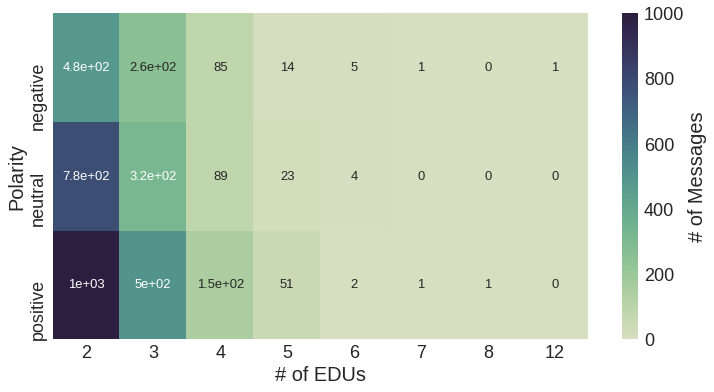
\includegraphics[width=\linewidth]{img/dasa_potts_edu_distribution.png}
      \caption{PotTS}\label{dasa:fig:data-distribution-potts}
    \end{subfigure}
  }
  \centering
  {
    \centering
    \begin{subfigure}{0.7\textwidth}
      \centering
      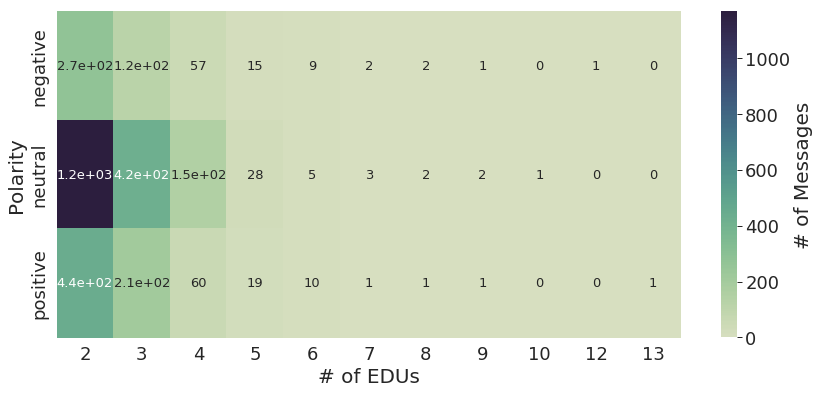
\includegraphics[width=\linewidth]{img/dasa_sb10k_edu_distribution.png}
      \caption{SB10k}\label{dasa:fig:data-distribution-sb10k}
    \end{subfigure}
  }
  \caption[EDU distribution in PotTS and SB10k]{Distribution of
    Elementary Discourse Units and Polarity Classes in the Training and
    Development Sets of PotTS and
    SB10k}\label{dasa:fig:data-distribution}
\end{figure*}

Figure~\ref{dasa:fig:data-distribution} shows the distribution of
elementary discourse units and polarity classes in the training and
development data of both dataset.  As we can see from these graphics,
the absolute majority of all tweets consist of maximally three
segments, whereas messages with more than five EDUs are extremely rare
and rather represent exceptions, which is not surprising regarding
that the maximum tweet length is constrained to at most 140
characters.  Nevertheless, in each corpus, we also can notice a few
microblogs with up to 12 or even 13 discourse units.  Since it was
somewhat unusual to see that many segments in a single microblog, we
decided to inspect these messages in more detail.  As it turned out,
such high numbers of EDUs typically arose from spurious punctuation
marks, which were apparently freely used in Twitter communication but
confused our segmenter.  You can see an example of such super-prolific
message in~\ref{dasa:exmp:many-segments}).

\begin{example}[SB10k Tweet with 13 EDUs]\label{dasa:exmp:many-segments}
  \noindent\textup{\bfseries\textcolor{darkred}{Tweet:}} { \upshape
    [Guinness on Wheelchairs :]$_1$ [Das .]$_2$ [Ist .]$_3$ [Verdammt
      .]$_4$ [Noch .]$_5$ [Mal .]$_6$ [Einer .]$_7$ [Der .]$_8$
    [Besten .]$_9$ [Werbespots .]$_{10}$ [Des .]$_{11}$ [Jahrzehnts
      .]$_{12}$ [( Auch ...]$_{13}$ }\\
    {\textup{[}Guinness on
      Wheelchairs :\textup{]$_1$} \textup{[}This .\textup{]$_2$}
    \textup{[}Is .\textup{]$_3$} \textup{[}Gosh .\textup{]$_4$}
    \textup{[}Darn .\textup{]$_5$} \textup{[}It .\textup{]$_6$}
    \textup{[}One .\textup{]$_7$} \textup{[}Of .\textup{]$_8$}
    \textup{[}The best .\textup{]$_9$} \textup{[}Commercials
      .\textup{]$_{10}$} \textup{[}Of .\textup{]$_{11}$} \textup{[}The
      Decade .\textup{]$_{12}$} \textup{[}( Also ...\textup{]$_{13}$}}
\end{example}

Another trend which we can observe from the data is that the
distribution of the polarity classes in the remained subset largely
reflects the frequencies of these semantic orientations in the
complete data: For example, the positive class still dominates the
PotTS corpus, while the neutral polarity constitues the vast majority
of the SB10k dataset.  Negative microblogs once again are the least
represented group in both cases and account for 22\% of the former
corpus and 16\% of the latter tweet set.

\todo[inline]{Describe RST Parser}

To obtain RST trees for the segemented messages, we \cite{Stede:14}

\citet{Bhatia:15}

\section{Discourse-Aware Sentiment Analysis}\label{sec:dasa:data}

% \done[inline]{\citet{Bickerstaffe:10}}

% \citet{Bickerstaffe:10} also considered the rating prediction task,
% addressing this problem with the minimum-spanning-tree (MST) SVM
% approach.  In the initial step of this method, they constructed a
% strongly connected graph whose vertices were associated with the most
% representative example (determined via the average all-pairs Tanimoto
% coefficient) of each star rating and the edge weights represented the
% Tanimoto distances between those nodes.  Afterwards, they determined
% the MST of this graph using the Kruskal's
% algorithm~\cite[see][pp.~567--574]{Cormen:09} and, finally,
% constructed a decision tree from this MST, replacing the MST vertices
% with binary SVM classifiers, which had to discern the respective
% rating groups. An evaluation on the four-star review corpus
% of~\citet{Pang:05} showed an improvement by up to~7\% over the
% previous state of the art, boosting it to 59.37\% average accuracy.


\done[inline]{\citet{Pang:02}}

\citet{Pang:02}, who experimented with three different approaches to
document-level sentiment analysis---Na{\"i}ve Bayes, Maximum Entropy,
and SVM with unigram and bigram features, pointed out that it was
insufficient to rely on the mere presence or majority of certain
polarity clues because these clues could any time be negated by a
single antithesis relation (see Example~\ref{disc-snt:exmp-pang02}
from \citet{Pang:02}).

\begin{example}[Polarity reversal via discourse antithesis]\label{disc-snt:exmp-pang02}
  \noindent\upshape This film should be brilliant.  It sounds like a
  great plot, the actors are first grade, and the supporting cast is
  good as well, and Stallone is attempting to deliver a good
  performance.  However, it can't hold up.
\end{example}

\done[inline]{\citet{Pang:04}}

One of the first approaches to coarse-grained sentiment analysis that
explicitly addressed discourse phenomena was presented
by~\citet{Pang:04}.  In their seminal work on predicting the semantic
orientation of movie reviews, the authors emphasized the need for
restricting the input to the polarity classifer to only subjective
sentences, ignoring objective ones which could easily confuse the
predictor.  To deal with this problem, they trained another
classification system which first assigned an initial subjectivity
value to every sentence in text; then constructed a graph, connecting
each sentential node to the nodes of its its neighbors and two
additional sink vertices representing the subjective and objective
classes; and, finally, devided this graph into two parts, allocating
all sentences to either of the two sinks and finding a minimum-cut
partition.

\done[inline]{\citet{Hu:04}, Section 3.6}

Similarly, \citet{Hu:04} in their work on mining and summarizing
customer reviews used discourse clues as a fallback strategy for
determining user's opinion about particular product features: The
authors first tried to determine the attitude toward a feature by
simply counting the number of postive and negative terms appearing in
the same sentence as the mentioned product aspect.  In case of a tie,
they resorted to counting these clues in the immeadiate nearby context
of the feature, and, if these also were equal, used the polarity of
the previous opinionated sentence, reversing it to the opposite if the
current sentence started with ``\emph{but}''.

\done[inline]{\citet{Mao:06}}

\citet{Mao:06} proposed the idea of isotonic CRFs in which they
explicitly modeled the constraint that features which were stronger
associated with either polarity classes had to have higher
coefficients than less predictive attributes.  After proving that this
formalism also allowed to directly model the ordinal scale of
sentiment scores (with lower CRF outputs indicating the negativity of
a sentence, and higher scores showing its positive class), the authors
used this approach to model the sentiment flow in a document.  For
this purpose, they first predicted the polarity value for each
sentence of a document in isolation and then convolved these outputs
with a Gaussian kernel, getting a smoothed polarity curve for the
whole analyzed text at the end.

\done[inline]{\citet{Polanyi:06}}

\citet{Polanyi:06} listed connectors and discourse relations among the
most important factors which could significantly change the intensity
and polarity of opinionated words.  They claimed that concessive links
between discourse segments might significantly weaken the strength of
an opinion, and, vice versa, elaborations on sentiments might notably
increase their persuasiveness.

\done[inline]{\citet{Thomas:06}}

\citet{Thomas:06} enhanced an SVM-based sentiment classification
system for predicting speaker's attitude in political speeches with
information about the inter-speaker agreement, incorporating these
links into the global cost function.  Thanks to this change, the
authors achieved $\approx$4\% improvement in accuracy (from 66.05 to
70.81\%) over the baseline classifer which analyzed each utterance in
isolation.

\done[inline]{\citet{McDonald:07,Sadamitsu:08}}

\citet{McDonald:07} proposed a joint framework for simultaneously
predicting the polarity of a document and its constituent parts (which
could be either paragraphs or sentences).  For this purpose, the
authors considered the semantic orientation of the whole text and its
single sentences as latent variables in a Markov random field,
connecting each unobserved sentence polarity node to the nodes of the
adjacent clauses as well as the overal polarity node of the complete
document, and then figuring out the best configuration of all
unobserved variables at the end.  With this method, they could
outperform both sentence- and document-level classifiers which
predicted the polarity classes of their input in isolation
(disregarding the context and hierarchical structure), and even
surpassed a cascaded system where the output of a sentence classifier
was fed into a document-level predictor, achieving 62.6\% sentence
accuracy (for three classes) and 82.8\% document-level precision (for
two classes) on a corpus of 600 reviews.  A similar approach was also
suggested by~\citet{Sadamitsu:08} who attained 82.74\% accuracy at
predicting the polarity class of customer reviews using hidden
conditional random fields and also looking for the most probable joint
configuration of sentence and document labels.

\done[inline]{\citet{Snyder:07}}

\citet{Snyder:07} proposed a Good Grief algorithm for jointly
predicting users' evaluations of different restaurant aspects.  For
this purpose, they first classified the attitude of the user to each
single predefined trait (food, ambience, service, etc.) and then
applied another clasifier in order to predict whether these scores
should rather agree or disagree with each other.  In the final step,
the authors looked for the ranking which best satisfied both of the
above predictions (i.e., ranks of individual aspects and their overall
agreement), achieving this way 0.632 ranking loss on a corpus of
$\approx$4,500 reviews and outperforming the renowned PRank algorithm
\cite{Crammer:01} which determined the rank for each aspect in
isolation.

\done[inline]{\citet{Voll:07}}

The effect of discourse phenomena was also pointed out by
\citet{Voll:07} who noted the fact that the mere occurrence of
positive or negative terms in a text was not necessarily indicative of
its main polarity if these terms appeared in off-topic sentences or
subordinate clauses.  To check this hypothesis, the authors compared
three different approaches to lexicon-based classification of customer
reviews:
\begin{inparaenum}[(i)]
\item by simply applying the SO-CAL system to all adjectives appearing in
the review,
\item by only taking into account those ones which appeared in the
  top-post nuclei of the sentences (as defined by the Rhetorical
  Structure Theory), and
\item by restricting the SO-CAL's input to clauses which had been
  previously preclassified as belonging to the main topic of the text.
\end{inparaenum}
They found the last option working best, yielding 73\% accuracy for
this two-class prediction task on the Epinion review corpus
of~\citet{Taboada:06}.  Unfortunately, the RST-based method did not
improve upon the baseline and resulted in only 69\% precision.  This,
however, might be partially due to the fact that the authors
completely ignored all nuclei and satellites within sentences except
for the main ones, did not consider the discourse relations between
the RST nodes, and also completely ignored all inter-sentential links.

\done[inline]{\citet{Somasundaran:08a,Somasundaran:08}}

\citet{Somasundaran:08a,Somasundaran:08} introduced the concept of
\emph{opinion frames} (OF)---special data structures for capturing the
relations between opinions in the discourse.  Depending on the type of
the opinions (either arguing~[\emph{A}] or sentiment~[\emph{S}]),
their polarity towards the targets (either positive~[\emph{P}] or
negative~[\emph{N}]), and semantic relationship between the two
targets (either alternative~[\emph{Alt}] or same~[\emph{same}]), they
distinguished 32 types of such frames: \emph{SPSPsame},
\emph{SPSNsame}, \emph{APAPalt}, etc., dividing them into reinforcing
and non-reinforcing ones; and also demonstrated the amenability of
this concept to automatic classification and its utility to
disambiguating the polarity of specific opinions.  Nevertheless, as
noted by the authors, OF and common discourse analysis frameworks,
although frequently going hand in hand, were not redundant to each
other, so that reinforcing frames could be expressed by both
contrastive and non-contrastive discourse relations, and vice-versa
non-reinforcing frames were not necessarily bound to a contrast in the
discourse.

\done[inline]{\citet{Somasundaran:09a,Somasundaran:09b}}

In a later work, \citet{Somasundaran:09b,Somasundaran:09a} also
introduced a joint inference framework based on the Iterative
Classification Algorithm (ICA) and Integer Linear Programming (ILP)
for joinly predicting the best configuration of single opinions and
their frames.  In this approach, the authors first applied a local SVM
classifier to compute the probabilities of polarity classes (positive,
negative, or neutral) of individual dialog acts and then harnessed the
ICA and ILP systems to determine which of the predicted opinions were
connected via opinion frames and whether these frames were reinforcing
or not.  Given a perfect information about the opinion links, this
joint method outperformed the local classifier by more than 9
percentage points, reaching 77.72\% accuracy on the AMI meeting
corpus~\cite{Carletta:05}.

\done[inline]{\citet{Asher:08}}

\citet{Asher:08} presented an annotation scheme and pilot corpus of
English and French texts labeled according to these guidelines, in
which they tried to explicitly take the SDRT theory as a basis for
sentiment representation.  For this purpose, the authors first asked
their annotators to analyze the segmented discourse structure of the
corpus texts and then ascribe one of the four major opinion categories
(reporting, judgement, advice, or sentiment) along with their
subcategories (e.g., inform, assert, blame, recommend) to each
discourse unit which featured at least one opinionated word from a
lexicon.  Afterwards, they showed that, with a simple set of rules,
one could easily propagate these opinions through the discourse
graphs, increasing the strengths or reversing the polarity of
sentiments depending on the type of discourse relations that connected
the segments.

\done[inline]{\citet{Yessenalina:10}}

Similarly, \citet{Yessenalina:10} proposed a latent-variable approach
in which they tried to predict the overall polarity of a document by
jointly selecting a subset of sentences which were most indicative of
document's semantic orientation and predicting the document's class
(either positive or negative) based on this subset.  To achieve this
goal, the authors adopted the latent-SVM method of \citet{Yu:09},
training a linear classifier on individual sentences with latent
classes and making the final prediction using 30\% of the sentences
which this classifier was most sure about.  To account for discourse
phenomena, they also enhanced feature representations of analyzed
sentences with attributes extracted from their preceding clauses and
added characteristics of the whole document to the model.  This way,
\citet{Yessenalina:10} attained 93.22\% accuracy on the movie review
corpus of \citet{Pang:04} and scored 77.09\% on the collection of
congressional floor debates introduced by \citet{Thomas:06}.

\done[inline]{\citet{Trivedi:13}}

Later on, \citet{Trivedi:13} refined this approach by introducing
special \emph{connector-augmented} transition features, which
reflected whether an explicit connector at the beginning of a sentence
implied a \emph{continuation} or \emph{shift} of the polarity of the
preceding discourse unit.  These attributes turned out to be extremely
useful, boosting the prediction accuracy on the movie review corpus
of~\citet{Maas:11} from 88.21 to 91.36\% in comparison with the
connector-unaware model.

\done[inline]{\citet{Heerschop:11}}

\citet{Heerschop:11} compared three different ways of incorporating
discourse information into a lexicon-based sentiment analysis system:
by increasing polarity scores of words that appeared near the end of
the document, by assigning higher weights to the tokens in the nuclei
of RST trees than its satellites, and, finally, by training a genetic
algorithm which learned separate coefficients for the nuclei and eight
types of satellite relations (\textsc{Attribution},
\textsc{Background}, \textsc{Cause}, etc.).  An evaluation of these
approaches on the movie review corpus of~\citet{Pang:04} showed the
superior performace of the first option (0.608 accuracy and 0,597
macro\F).  However, after adding an offset to the decision boundary
(accounting for the fact that negative reviews could contain multiple
positive terms) significantly improved the results of the last
classifier, which eventually outperformed all other competitors,
yielding 0.72 accuracy and macro-averaged~\F.

\done[inline]{\citet{Zhou:11}}

\citet{Zhou:11} used automatically derived RST trees to disambiguate
the polarity of complex sentences which contained both positive and
negative terms.  To determine the semantic orientation of the whole
sentence, the authors applied a set of heuristic rules that described
possible polarity changes of elementary discourse units based on their
nucleus/satellite-status and discourse relation connecting them to the
parent.  With these rules, \citeauthor{Zhou:11} attained a
statistically significant improvement in sentence-level polarity
classification on the NTCIR MOAT corpus~\cite{Xu:10}, successfully
resolving more than a half of ambiguities.

\done[inline]{\citet{Zirn:11}}

An approach which probably comes closest to ours was proposed
by~\citet{Zirn:11}, who used a lexicon-based sentiment system to
compute polarity scores of elementary discourse units, and then
applied a set of Markov logic rules to enforce consistency of these
polarity assignments over an automatically derived RST tree.  Apart
from experimenting with tree structures, the authors also checked
whether simply preferring the same semantic orientation for linearly
adjacent segements would improve the accuracy.  Surprisingly, this
latter option worked the best, achieving 69.02\% accuracy on the
Amazon review dataset of~\citet{Blitzer:07} and significantly
outperforming both discourse-unaware and RST-tree--based baseline
classifiers.

\done[inline]{\citet{Wang:13},\citet{Chenlo:13,Chenlo:14}}

Another RST-based framework was proposed by~\citet{Wang:13} who also
computed polarity scores of elementary discourse segments, and
determined the polarity of the whole document by computing a linear
combination of these scores multiplied with their doscourse
coefficients.  These coefficients were learned automatically during
training and, similarly to the approach of~\citet{Zirn:11}, depended
on the status of the segment in the RST tree (either nucleus or
sattelite) and the relation connecting it to the ancestor node.  Using
a restricted subset of such relations (\textsc{Contrast},
\textsc{Cause}, \textsc{Generalization}, and \textsc{Condition}), the
authors achived a considerable improvement over the baseline system in
which all segments were weighted equally (0.8528 versus 0.8386\F).  A
similar method was also used by \citet{Chenlo:13,Chenlo:14} for
analyzing blog posts, where it also proved its efficiency, leading to
much better results than discourse-unaware baselines.

\done[inline]{\citet{Bhatia:15}}

Other ways of incorporating discourse structure into an opinion mining
application were proposed by~\citet{Bhatia:15} who presented two
methods for augmenting a sentiment analysis system with discourse
information:
\begin{inparaenum}[(i)]
\item discourse depth reweighting (DDR) and
\item rhetorical recursive neural network (R2N2).
\end{inparaenum}

In the former approach, the authors first computed the sentiment score
$\lambda_i$ of each elementary discourse unit $i$ as:
\begin{equation*}
  \lambda_i = \max\left(0.5, 1 - d_i/6\right),
\end{equation*}
where $d_i$ stands for the depth of the $i$-th EDU in the discourse
tree of the whole document.  Afterwards, they estimated the overall
polarity of the document~$\Psi$ by summing up the linear predictions
for each discourse unit ($\theta^T\cdot\mathbf{w}_i$), scaling these
prediction by the factor~$\lambda_i$:
\begin{equation*}
  \Psi = \sum_i\lambda_i\mathbf{\theta}^T\cdot\mathbf{w}_i = \mathbf{\theta}^T\cdot\sum_i\lambda_i\mathbf{w}_i,
\end{equation*}
In this equation, $\mathbf{\theta}$ represents a vector of polarity
scores ($-1$ for negative terms and $+1.$ for positive entries) for
all word in the vocabulary (as obtained from the sentiment lexicon
of~\citet{Wilson:05}), and $w_i$ denotes the bag-of-words
representation of the $i$-th EDU.

In the R2N2 method, \citet{Bhatia:15} adopted the RNN approach
of~\citet{Socher:13} and recursively computed polarity scoreb of each
discourse $i$ unit as follows:
\begin{equation*}
  \psi_i = tanh\left(K_n^{(r_i)} \psi_{n(i)} + K_s^{(r_i)}\psi_{s(i)} \right),
\end{equation*}
where $K_n^{(r_i)}$ and $K_s^{(r_i)}$ denote the nucleus an satellite
coefficients associated with the rhetorical relation $(r_i)$, and
$\psi_{n(i)}$ and $\psi_{s(i)}$ represent the sentiment scores of the
nucleus and satellite nodes of the $i$-th discourse unit.  With this
method, the authors achieved 84.1\% two-class prediction accuracy on
the moview review corpus of~\citet{Pang:04} and 85.6\% on the dataset
of~\citet{Socher:13}.

\done[inline]{Others}

\done[inline]{\citet{Riloff:03}}

\citet{Riloff:03} added a set of discourse-related features, such as
relative sentence lengths, the average number of subjective clues in
the preceding, current, and following clauses, and the relative number
of these clues with respect to the corresponding sentence lengths,
getting more than 2\% accuracy improvement over a baseline Na{\"i}ve
Bayes classifier which did not utilize this information.

\section{Evaluation}

\subsection{Relation Scheme}

\begin{table}[h]
  \begin{center}
    \bgroup \setlength\tabcolsep{0.1\tabcolsep}\scriptsize
    \begin{tabular}{p{0.17\columnwidth} % first columm
        *{1}{>{\centering\arraybackslash}p{0.4\columnwidth}}
        *{1}{>{}p{0.4\columnwidth}}} % next two columns
      \toprule
      \textbf{Authors} & \textbf{Relation Set} & \textbf{Equivalence Classes}\\\midrule

      \citet{Heerschop:11} & \{\textsc{Attribution},
      \textsc{Background}, \textsc{Cause}, \textsc{Condition},
      \textsc{Contrast}, \textsc{Elaboration}, \textsc{Enablement},
      \textsc{Explanation}, \textsc{\bfseries Other}\} & \\

      \citet{Zhou:11} & \{\textsc{Contrast}, \textsc{Condition},
      \textsc{Continuation}, \textsc{Cause}, \textsc{Purpose},
      \textsc{\bfseries Other}\} & \textsc{Contrast} $\defeq$
      \{\textsc{Antithesis}, \textsc{Concession}, \textsc{Otherwise},
      \textsc{Contrast}\};\newline \textsc{Continuation} $\defeq$
      \{\textsc{Continuation}, \textsc{Parallel}\};\newline
      \textsc{Cause} $\defeq$ \{\textsc{Evidence}, \textsc{Volitional
        Cause}, \textsc{Nonvolitional-Cause},
      \textsc{Volitional-Result}, \textsc{Nonvolitional-Result}\};\\

      \citet{Chenlo:13} & \{\textsc{Attribution}, \textsc{Background},
      \textsc{Cause}, \textsc{Comparison}, \textsc{Condition},
      \textsc{Consequence}, \textsc{Contrast}, \textsc{Elaboration},
      \textsc{Enablement}, \textsc{Evaluation}, "Explanation",
      \textsc{Joint}, \textsc{Otherwise}, \textsc{Temporal},
      \textsc{\bfseries Other}\} & \\

      \citet{Bhatia:15} & \{\textsc{Contrastive},
      \textsc{\bfseries Non-Contrastive}\} & \textsc{Contrastive} $\defeq$
      \{\textsc{Antithesis}, \textsc{Antithesis-E},
      \textsc{Comparison}, \textsc{Concession},
      \textsc{Consequence-S}, \textsc{Contrast},
      \textsc{Problem-Solution}\}.\\\bottomrule
\end{tabular}
    \egroup
    \caption[RST relations used in different discourse-aware sentiment
      methods]{RST relations used in different discourse-aware
      sentiment methods\\ {\small (default relation [which subsumes
          the rest of the links] is highlighted in
        \textbf{boldface})}}
    \label{dasa:tbl:rst-rels}
  \end{center}
\end{table}

\section{Summary and Conclusions}
